\section{Introduction}

The prevailing opinion is that the traditional use of bootstrapping to produce confidence intervals for penalized regression is suboptimal due to the inherent behavior of estimates produced by penalization.

Specifically, we see two potential problems that arise when proposing to use bootstrapping for penalized regression, we will refer to these obstacles as,

\begin{enumerate}
\item the shrinkage problem, and
\item the point mass problem.
\end{enumerate}

The shrinkage problem refers to the bias introduced by penalization. This penalization leads to coverages much higher than nominal coverage rates for coefficients with true values at or very near zero and leads to much lower coverage when coefficients are non-zero. We argue that coverage in the traditional sense is too ridged of a paradigm to apply to penalized regression inference. Instead, we offer a different perspective and argue that the impact that penalization induced bias has is an inherent feature of penalized regression rather than a flaw. Since high dimensional problems often necessitate such an alternate approach, we offer guidance on how to interpret the confidence intervals for lasso as presented in this paper.

The second problem, the point pass problem, is related to the shrinkage problem but arises as an arguably more disturbing manifestation: confidence intervals of length zero. Some penalized regression methods, particularly the lasso, often results in a sparse solution. If using a traditional quantile based bootstrap confidence interval, this will lead to an interval of [0,0] if a given variable is rarely or never included in the model \logan{Maybe this is better termed "active set" or "selected"}. As the dimensionality of the problem grows, this becomes an increasing occurrence leading to a large majority of intervals possessing a length of zero. When the true value of the coefficient is 0, the interval at least contains the truth. However, this issue is particularly troublesome when one considers what happens when the true value is not precisely zero, as is likely the case in most reasonable scenarios. By just shifting the true value by $\eps$, an immediate drop in coverage would occur.

The later of these two problems is addressed in our novel approach to producing bootstrap based confidence intervals for the lasso.

\section{Empirical Bayes Bootstrap Confidence Intervals}

As with other penalized regression models, the lasso can be formulated as a Bayesian regression model by setting an appropriate prior. For the lasso, this prior is a Laplace, also called double-exponential, distribution:

\as{\p(\bb) = \prod_{j = 1}^{p} \frac{\gamma}{2}\exp(-\gamma \abs{\beta_j}), \gamma > 0}

With this prior, the lasso estimate $\bbh(\lam)$ is the posterior mode of $\bb$ when $\lam = \gamma \frac{\sigma^2}{n}$.

We propose leveraging this relationship to build confidence intervals for $\bb$. Specifically, we propose the following process for given values of $\lam$, $\sigma^2$, and significance level, $\l$:

\begin{enumerate}
\item Obtain a bootstrap sample of $\X$ and $\y$
\item For each $\beta_j$:
	\begin{enumerate}
	\item Obtain the marginal posterior for $\beta_j$
	\item Compute the quantiles for $p_{L} = (.5 - \l/2)$ and $p_{U} = (.5 + \l/2)$ and save
	\end{enumerate}
\item Repeat $\m$ times
\item For each $\beta_j$, take the average of the $\m$ lower and upper quantiles to produce a final confidence interval estimate
\end{enumerate}

\section{Details}

In this section, we describe the details of each of the steps outlined above along with other important considerations.

\subsection{Bootstrap Sampling}

There are various ways to perform a single iteration of a bootstrap, among them are the pairs bootstrap and the residual bootstrap. For high dimensional problems in general, the pairs bootstrap is attractive. First, it makes the fewest assumptions compared to other methods. Specifically, the only assumption made for the pairs bootstrap is that the original pairs were randomly sampled from some distribution $F$, where $F$ is a distribution on (p + 1)-dimensional vectors (Efron, Tibshirani). Additionally, the pairs bootstrap is simple to perform. Finally, and perhaps most importantly, it treats $\X$ as random which is almost surely the case in high dimensional settings. For this reason, we will solely focus on and use the pairs bootstrap in our proposed procedure.

\subsection{Obtaining Intervals}

\subsubsection{Computing the marginal posterior for \texorpdfstring{$\beta_j$}{betaj}}

\logan{Say something about focus on marginal? Use of partial residuals?}

Unfortunately, a Normal likelihood and Laplace prior are not conjugate and in general, the absolute value in the exponent of the Laplace makes many common manipulations for the posterior more difficult. Luckily, however, the marginal posterior can be shown to be a mixture of a right and left truncated normal where the truncation occurs at zero for right and left tails respectively. To obtain a marginal posterior, we use the partial residuals, $\r_{-j}$, in the likelihood. In the steps that follow, we will assume that $\X$ has been standardized s.t. $\x_j^T\x_j = n$. For $\beta_j$,

\as{
L(\beta_j | \r_{-j}) &= (\sigma \sqrt{2\pi})^{-n} \exp(-\frac{1}{2\sigma^2} (n\beta_j^2 - 2\x_{j}^{T}\r_{-j}\beta_j + \r_{-j}^{T}\r_{-j})) \\
&\propto \exp(-\frac{n}{2\sigma^2} (\beta_j^2 - 2z_j\beta_j)), \text{ where } z_{j} = \frac{1}{n} \x_{j}^{T}\r_{-j} \\
\Rightarrow P(\beta_j | \r_{-j}) &\propto \exp(-\frac{n}{2\sigma^2} (\beta_j^2 - 2z_{j}\beta_j)) \frac{n \lambda}{2 \sigma^2} \exp(-\frac{n \lambda} {\sigma^2} \abs{\beta_j}) \\
&\propto \exp(-\frac{n}{2\sigma^2} (\beta_j^2 - 2 z_j\beta_j +  2 \lambda \abs{\beta_j})) \\
&= \exp(-\frac{n}{2\sigma^2} (\beta_j^2 - 2(z_j\beta_j - \lambda \abs{\beta_j}))) \\
&=
\begin{cases}
\exp(-\frac{n}{2\sigma^2} (\beta_j^2 - 2(z_j + \lambda)\beta_j)), \text{ if } \beta_j < 0, \\
\exp(-\frac{n}{2\sigma^2} (\beta_j^2 - 2(z_j - \lambda)\beta_j )), \text{ if } \beta_j \geq 0 \\
\end{cases} \\
&\propto
\begin{cases}
C_{-} \exp(-\frac{n}{2\sigma^2} (\beta_j - (z_j + \lambda))^2), \text{ if } \beta_j < 0, \\
C_{+} \exp(-\frac{n}{2\sigma^2} (\beta_j - (z_j - \lambda))^2), \text{ if } \beta_j \geq 0 \\
\end{cases}
}

Where, $C_{-} = \exp(\frac{z_j \lambda n}{\sigma^2})$ and $C_{+} = \exp(-\frac{z_j \lambda n}{\sigma^2})$.

Ignoring the truncation for a moment and focusing on the kernels individually, we can see that the two distributions above are what we would expect from the lasso solution, having a mean $z_j + \lambda$ and $z_j - \lambda$ respectively and a variance of $\frac{\sigma^2}{n}$. That said, due to the truncation, the variance of the posterior is less than or equal to this (plot the marginal posterior and this should become immediately clear). Furthermore, a mapping allows tail probabilities from the posterior to be translated to probabilities onto corresponding known normal distributions ($\N(0, z_j \pm \lambda, \frac{\sigma^2}{n})$). For this translation, we need two pieces of information:

\begin{enumerate}
\item The non-truncated probability in each of the two normals to transformed on to, denoted $Pr_{-}$ and $Pr_{+}$ respectively.
\item The probability in each of the tails of the posterior, denoted $Post_{-}$ and $Post_{+}$ respectively.
\end{enumerate}

(1) is trivial to compute with any statistical software. Similarly, (2) is conceptually simple, although care must be taken to avoid the pitfall of numerical instability introduced as n increases. \logan{Not sure how much more detail to get into, I think it is common enough?}

To reduce the number of computational steps, one may note that:

\as{
P(\beta_j | \r_{-j})  & \propto
\begin{cases}
C_{-} Pr_{-}, \text{ if } \beta_j < 0, \\
C_{+} Pr_{+}, \text{ if } \beta_j \geq 0 \\
\end{cases}
}

Which implies that $Post_- = \frac{C_{-} Pr_{-}}{C_{-} Pr_{-} + C_{+} Pr_{+}}$ and similarly for $Post_+$. However, to avoid numerical instability, or at least handle it properly when it is unavoidable we need to work on the $\log$ scale. This works well for most of the problem, but computation of $Post_-$ and $Post_+$ need something a bit more since, for example, $\log(Post_-) = \log(C{-}Pr_{-}) - \log(C_{-} Pr_{-} + C_{+} Pr_{+})$. That is, the denominator still must be computed then the $\log$ taken which does not allow operating on the $\log$ scale to fully address potential instability. Instead, $\log(Post_-)$ can be computed with $\log(Pr_-) + \log(C_-) -  \log(Pr_+) + \log(C_+) - \log(1 + \exp(\log(Pr_-) + \log(C_-) -  \log(Pr_+) + \log(C_+)))$. \logan{CONTINUE HERE}.

With these values, we can compute quantiles by mapping the corresponding probabilities of interest $p_{L}$ and $p_{U}$ for the posterior onto the probabilities $p^*_{L}$ and $p^*_{U}$ for the corresponding normals. Which normal the quantiles of interest ultimately come from is determined based on the values in (2). For example, if $Post_{+} = .98$ and $\l = .8$ ($p_{L} = .1$ and $p_{U} = .9$), then both $p_{L}$ and $p_{U}$ would be mapped onto the positive normal. As one more example, say $Post_{+} = .4$, then $p_{L}$ would be mapped onto the lower normal and $p_{U}$ would be mapped onto the upper normal. The transformation to map a given probability from the posterior depends on which tail the quantile resides in on the posterior (equivalently which normal it is being mapped to, the positive or negative). This map is:

\as{
p^* &= p \times (Pr_{\pm} / Post_{\pm}) \\
}

Once this respective probabilities are mapped, one can simply use the inverse of the normal CDFs that the probabilities were mapped to. That being said, there is a nuance worth pointing out. When transforming the probabilities, the step to determine which tail the respective quantile comes from occurs first. With this, the probability should be adjusted so that it refers to the probability between the quantile of interest and the respective tail. After this, then the transformation can be applied.

\logan{Need a better term for the two halves than tail....}

This solution corresponds to a particular value of $\lam$ and $\hat{\sigma}^2$. The only thing prohibitive to producing intervals for the entire lasso path is computational resources since the bootstrap is already computationally expensive. That brings our decision down to producing an estimate for $\sigma^2$. Our recommendation is to first use cross validation (CV) once to produce an estimate. However, note that producing an estimate in this manner implicitly depends on $\lam$, so new estimates for $\sigma^2$ should be obtained for each value of $\lam$.

\logan{Recommendation for $\lam$? How to actually use this? Personally, I imagine this method to be used as: }

Our recommendation is to use CV to select $\lam$ and produce an estimate for $\sigma^2$ and produce bootstrap confidence intervals corresponding to these values to report.

\logan{Not sure how much focus to put on the conceptual method vs. what actually is being done}

All together this leads to the following steps to perform the bootstrap:

\begin{enumerate}
\item Perform CV using the original data to select $\lam$ and estimate $\hat{\sigma}^2(\lam)$
\item For i $\in \lbrace 1 \ldots m \rbrace$:
\begin{enumerate}
\item Obtain a pairs bootstrap sample, $\X^*$ and $\y^*$
\item Fit lasso with $\X^*$ and $\y^*$
\item For j $\in \lbrace 1 \ldots p \rbrace$:
	\begin{enumerate}
	\item Obtain the partial residuals, $r_{-j}$ and compute $z_j$
	\item Compute $Pr_{-}$ = $\Phi(0, z_j + \lam, \frac{\sh^2}{n})$ and $Pr_{+}$ = $1 - \Phi(0, z_j - \lam, \frac{\sh^2}{n})$
	\item Compute $Post_-$ and $Post_+$
	\item For $p_L$ and $p_U$:
	\begin{algorithmic}
		\If {$p_* \leq P_{-} / A_{-}$}
			\State $q_* = \Phi^{-1}(p_* A_{-}, z_j + \lam, \frac{\sh^2}{n})$
		\Else
			\State $q_* = \Phi^{-1}(1 - (1 - p_*)A_{+}, z_j - \lam, \frac{\sh^2}{n})$
		\EndIf
	\end{algorithmic}
	\item Save $q_L$ and $q_U$
	\end{enumerate}
\end{enumerate}
\item For each $\beta_j$, take the average of the $\m$ lower and upper quantiles to produce a final confidence interval estimate
\end{enumerate}

\section{Simulation Studies}

\subsection{Overall vs. per-feature coverage}

\subsection{Across \texorpdfstring{$\lambda$}{lambda} Performance}
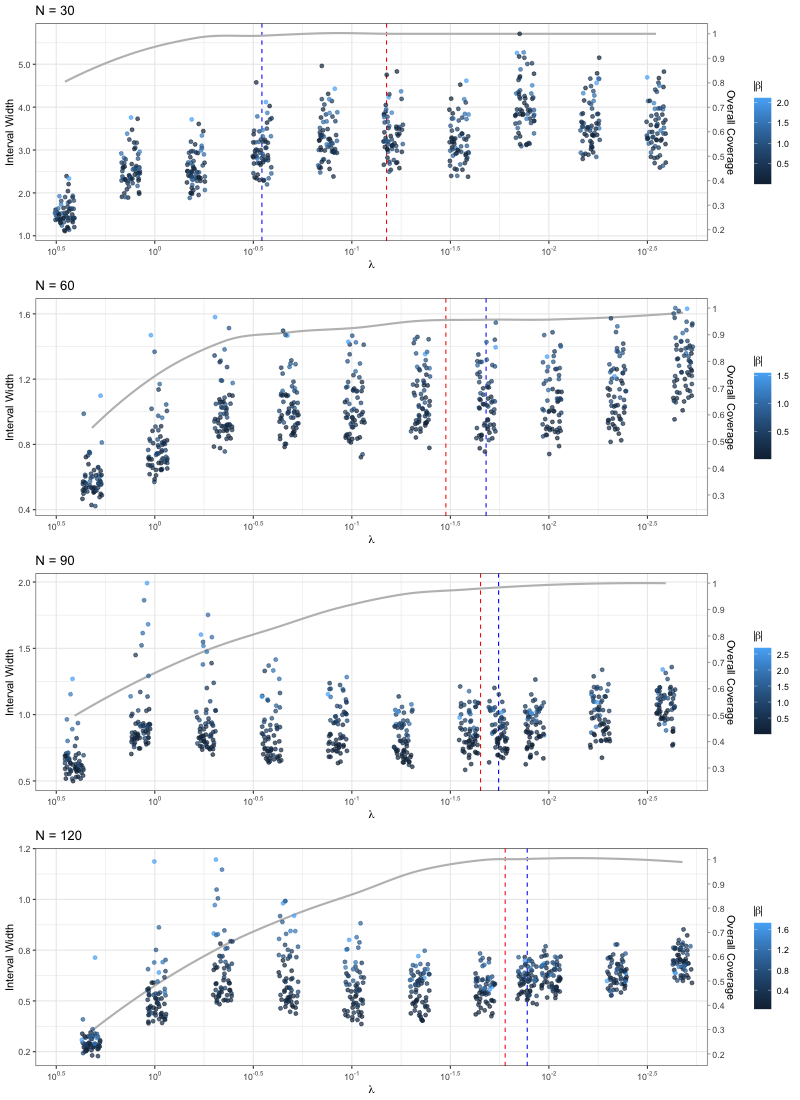
\includegraphics[width=\linewidth]{across_lambda_coverage_laplace.pdf}

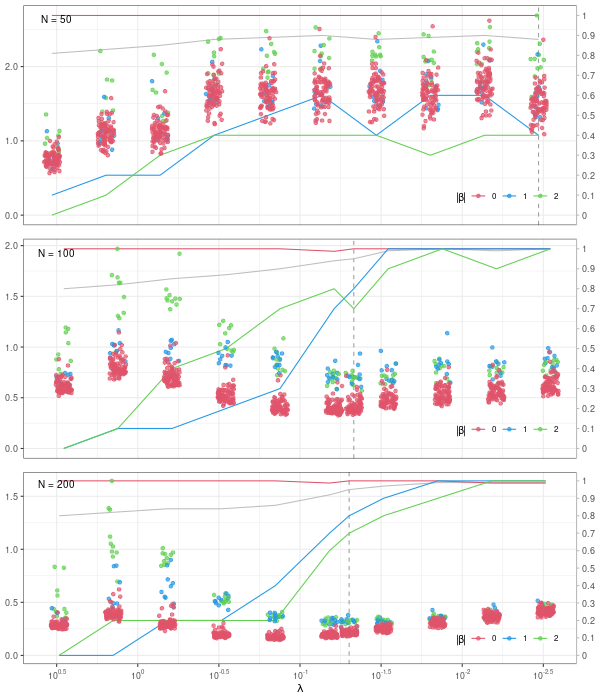
\includegraphics[width=\linewidth]{./fig/tmp/across_lambda_coverage_sparse.pdf}

\subsection{Distribution of Beta}

Sparse vs. dense, may not need? Or just show general patterns are the same?

\subsection{Epsilon Conundrum (Comparison to Traditional Quantile Bootstrap)}
\includegraphics[width=\linewidth]{./fig/tmp/bootstrap_quantile_comparison.pdf}

\subsection{Correlated Features (Comparison to Ridge)}


\subsection{Comparison to Other Methods}

\begin{enumerate}
\item Selective inference
\begin{enumerate}
\item Does not work for $p > n$ case
\item Only produced CI for variables in active set
\item Seems cumbersome and unstable as implemented
\item Unclear recommended selection of $\lam$
\item Non-finite endpoints not uncommon
\end{enumerate}
\item{Bootstrap Lasso Projection}
\end{enumerate}

\section{Citation Example}
\cite{Tibshirani1996} (the example citation) is now working


\section{Real data}

\section{Conclusions}

\section*{Acknowledgments}

\section*{Appendix}
